\documentclass[submit]{harvardml}

% FDV: Make sure all front matter has correct years, dates, book sections, etc.
\course{CS181-S22}
\assignment{Assignment \#2}
\duedate{7:59pm EST, Feb 25th, 2022}

\usepackage[OT1]{fontenc}
\usepackage[colorlinks,citecolor=blue,urlcolor=blue]{hyperref}
\usepackage[pdftex]{graphicx}
\usepackage{subfig}
\usepackage{fullpage}
\usepackage{amsmath}
\usepackage{amssymb}
\usepackage{framed}
\usepackage{color}
\usepackage{soul}
\usepackage{todonotes}
\usepackage{listings}
\usepackage{common}
\usepackage{enumitem}
\usepackage{bm}
\newcommand{\B}{\text{B}}
\newcommand{\Beta}{\text{Beta}}

\usepackage[mmddyyyy,hhmmss]{datetime}

\definecolor{verbgray}{gray}{0.9}

\lstnewenvironment{csv}{%
  \lstset{backgroundcolor=\color{verbgray},
  frame=single,
  framerule=0pt,
  basicstyle=\ttfamily,
  columns=fullflexible}}{}

\begin{document}

\begin{center}
{\Large Homework 2: Classification and Bias-Variance Trade-offs}\\
\end{center}

\subsection*{Introduction}

This homework is about classification and bias-variance trade-offs. In
lecture we have primarily focused on binary classifiers trained to
discriminate between two classes. In multiclass classification, we
discriminate between three or more classes.  Most of the material for Problem 1 and Problem 3, and all of the material for Problem 2 will be covered by the end of the Tuesday 2/8 lecture. The rest of the material will be covered by the end of the Thursday 2/10 lecture.  We encourage you to read
CS181 Textbook's Chapter 3 for more information on linear
classification, gradient descent, classification in the discriminative
setting (covers multiclass logistic regression and softmax), and
classification in the generative setting. Read Chapter 2.8 for more
information on the trade-offs between bias and variance.

As a general note, for classification problems we imagine that we have
the input matrix $\boldX \in \reals^{N \times D}$ (or perhaps they
have been mapped to some basis $\bm{\Phi}$, without loss of
generality) with outputs now ``one-hot encoded."  This means that if
there are~$K$ output classes, rather than representing the output
label $y$ as an integer~${1,2,\ldots,K}$, we represent $\boldy$ as a
``one-hot" vector of length~$K$. A ``one-hot" vector is defined as
having every component equal to 0 except for a single component which
has value equal to 1.  For example, if there are $K = 7$ classes and a
particular data point belongs to class 3, then the target vector for
this data point would be~$\boldy = [0,0,1,0,0,0,0]$.  We will define
$C_1$ to be the one-hot vector for the 1st class, $C_2$ for the 2nd
class, etc.  Thus, in the previous example $\boldy = C_3$. If there
are $K$ total classes, then the set of possible labels is $\{C_1
\ldots C_K \} = \{C_k\}_{k=1}^K$.  Throughout the assignment we will
assume that each label $\boldy \in \{C_k\}_{k=1}^K$ unless otherwise
specified. The most common exception is the case of binary classification
($K = 2$), in which case labels are the typical integers $y \in \{0, 1\}$.\\

In problems 1 and 3, you may use \texttt{numpy} or \texttt{scipy}, but
not \texttt{scipy.optimize} or \texttt{sklearn}. Example code given is
in Python 3.\\

Please type your solutions after the corresponding problems using this
\LaTeX\ template, and start each problem on a new page.\\

Please submit the \textbf{writeup PDF to the Gradescope assignment `HW2'}. Remember to assign pages for each question.  \textbf{You must include your plots in your writeup PDF. } The supplemental files will only be checked in special cases, e.g. honor code issues, etc. \\

Please submit your \textbf{\LaTeX\ file and code files to the Gradescope assignment `HW2 - Supplemental'}. 

%%%%%%%%%%%%%%%%%%%%%%%%%%%%%%%%%%%%%%%%%%%%%
% Problem 1
%%%%%%%%%%%%%%%%%%%%%%%%%%%%%%%%%%%%%%%%%%%%%

\begin{problem}[Exploring Bias and Variance, 10 pts]
  In this problem, we will explore the bias and variance of a
  few different model classes when it comes to logistic regression.

  Consider the true data generating process $y \sim \text{Bern}(f(x)), f(x) = 0.4 \times \sin(1.2x) + 0.5$, where $x \in [-3, 3]$, and $y \in \{0,1\}$.
  Recall that for a given $x$, bias and variance are defined in terms of expectations \textit{over randomly drawn datasets} $D$
  from this underlying data distribution:
  \begin{align*}
  \text{Bias}[\hat{f}(x)] &= \mathbb{E}_D[\hat{f}(x)] - f(x)\\
  \text{Variance}[\hat{f}(x)] &= \mathbb{E}_D[(\hat{f}(x) - \mathbb{E}_D[\hat{f}(x)])^2]
  \end{align*}
  Here, $\hat{f}(x)$ is our estimator (learned through logistic
  regression on a given dataset $D$).  We will directly explore the
  bias-variance trade-off by drawing multiple such datasets and
  fitting different logistic regression models to each.  Remember that
  we, the modelers, do not usually see the true data distribution.
  Knowledge of the true $f(x)$ is only exposed in this problem to (1)
  make possible the simulation of drawing multiple datasets, and (2)
  to serve as a pedagogical tool in allowing verification of the true
  bias.

\begin{enumerate}

\item Consider the three bases $\phi_1(x) = [1, x]$, $\phi_2(x) = [1,
  x, x^2]$, $\phi_3(x) = [1, x, x^2, x^3, x^4, x^5]$.  For each
  of these bases, generate 10 datasets of size $N = 30$ using the
  starter code provided, and fit a logistic regression model using
  sigmoid($w^T \phi(x)$) to each dataset by using gradient descent to
  minimize the negative log likelihood.  This means you will be
  running gradient descent 10 times for each basis, once for each
  dataset.  Note that the classes are represented with 0's and 1's.
  
  Use random starting values of $w$, $\eta=0.001$, take 10,000 update
  steps for each gradient descent run, and make sure to average the
  gradient over the data points (for each step). These parameters,
  while not perfect, will ensure your code runs in a reasonable amount
  of time. The emphasis of this problem is on capturing the
  bias-variance trade-off, so don't worry about attaining perfect
  precision in the gradient descent as long as this trade-off is
  captured in the final models.

   Note: Overflow RuntimeWarnings due to \verb|np.exp| should be safe to ignore, if any. Also, to reduce stress from randomness in students' solutions (due to randomized weight initialization differences), in line $109$ of the \verb|T2_P1.py| starter code, we call \verb|np.random.seed(1738)| to set a deterministic random seed. Please do not change this! In addition, please do not change the randomized weight initialization code in lines $42-46$.

\item Create three plots, one for each basis. Starter code is available which you may modify.
By default, each plot displays three types of functions:
(1) the true data-generating distribution $f(x)$ (the probability that $y=1$ for different $x$).
(2) all 10 of the prediction functions learned from each randomly drawn dataset, and
(3) the mean of the 10 prediction functions.
Moreover, each plot also displays 1 of the randomly generated datasets and highlights the corresponding prediction function learned by this dataset.

\item How are bias and variance reflected in the 3 types of curves on
  the graphs?  How do the fits of the individual and mean prediction
  functions change?  Keeping in mind that none of the model classes
  match the true generating process exactly, discuss the extent to
  which each of the bases approximates the true process.

  Note: In this problem, we are not interested in whether the model is
  more biased for certain inputs $x$ compared to other inputs $x'$.
  We are interested in the overall bias and variance of $\hat{f}(x)$
  across the different basis choices. In other words, we want to investigate how the bias between $\hat{f}(x)$ and the ground truth as well as the variance of $\hat{f}(x)$ will be different over different basis choices. 

\item If we were to increase the size of each dataset drawn from $N = 30$ to a larger number, how would the variance change? The bias?   Why might this be the case?

\end{enumerate}

\end{problem}

\newpage

\subsection*{Solution 1.2:}
\begin{center}
    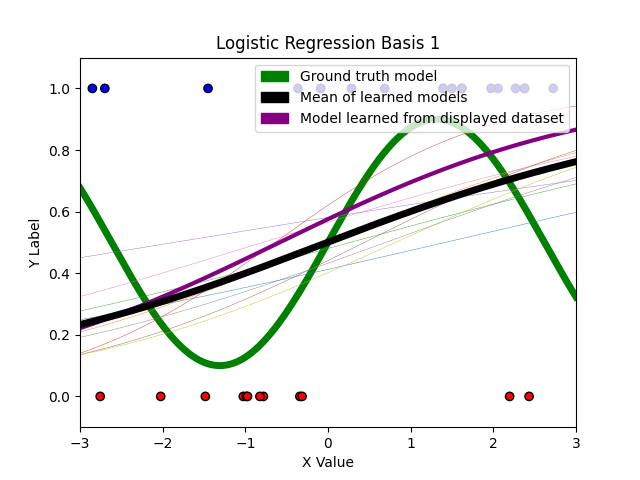
\includegraphics[scale = 0.75]{Logistic Regression Basis 1.png} \\
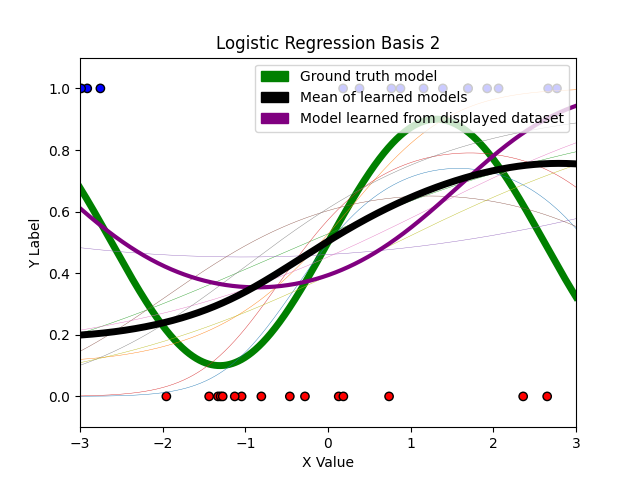
\includegraphics[scale = 0.75]{Logistic Regression Basis 2.png} \\
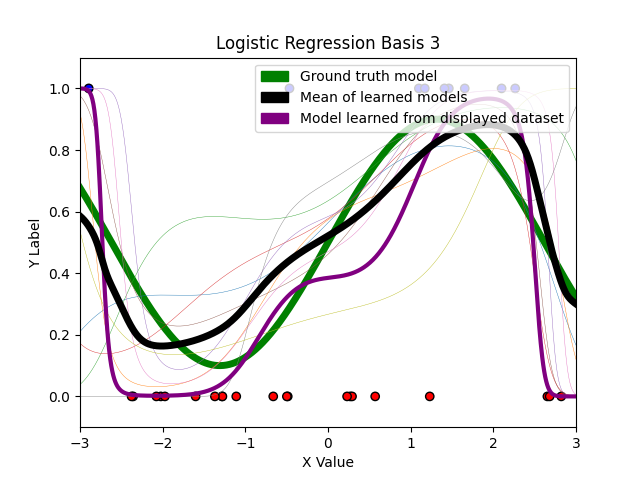
\includegraphics[scale = 0.75]{Logistic Regression Basis 3.png}
\end{center}

\subsection*{Solution 1.3:}
Looking at the graph for each basis, it appears that going in increasing order of basis functions (basis 1, basis 2, basis 3), bias decreases while variance increases. 
\\ \\
Looking at the graph corresponding basis 1, we see that the curve representing the mean of learned models is almost linear. With this basis, bias is very high as the models have little to no response towards variation in the data, leading the model to fit a generalized shape of the ground truth model. At the same time, variance in the models produced by this basis function are very low and all 10 models appear for the most part homogeneous. Overall, the models created by this basis function underfit the ground truth model.
\\ \\
Looking at the graph corresponding basis 2, we see that the curve representing the mean of learned models has a shape more similar to the ground truth model than basis 1. This can be attributed to reduced bias, as the learned models are more responsive to change in the data. At the same time, this leads to higher variance amongst learned models, as can be seen by the higher disparity between the mean of learned models and the model learned from the displayed dataset and between different learned models in general. Overall this basis function fits the ground truth model reasonably well and is a medium between basis 1 and basis 3 in terms of bias and variance.
\\ \\
Finally, looking at the graph for basis 3, we see that the curve representing the mean of learned models follows the ground truth model with fairly good accuracy. This is because of low bias, causing the learned models to be very responsive to the dataset. However, while this basis function generates models whose mean closely models the ground truth, there is the highest level of variance as the learned models respond very dramatically to the randomly drawn datasets from which they are trained. Overall, this leads this basis function to create models which overfit the model and may not generalize well to new data points.

\subsection*{Solution 1.4:}
If we were to increase the size of each dataset drawn to a larger number, variance would definitely decrease. Variation between larger datasets would be on average lower as the overall trends of these datasets would more accurately represent the ground truth model. As such, the variance of generated models would decrease as datasets would be more similar. At the same time, bias would not change significantly but might decrease slightly in response to an increase in the size of each dataset. Bias appears to be affected more by the basis used than the size of the dataset drawn. For example, if we were to increase the size of the dataset used for Basis 1, we would not significantly decrease bias as the basis does not have a high enough dimensionality to model the ground truth in a highly specific manner. Potentially, in the case of Basis 3, with an increase of size in the dataset, the overall trend of the dataset would more closely resemble ground truth, allowing generated models to have lower bias.
%%%%%%%%%%%%%%%%%%%%%%%%%%%%%%%%%%%%%%%%%%%%%
% Problem 2
%%%%%%%%%%%%%%%%%%%%%%%%%%%%%%%%%%%%%%%%%%%%%

\begin{problem}[Maximum likelihood in classification, 15pts]

  Consider now a generative $K$-class model.  We adopt class prior
  $p(\boldy = C_k; \bpi) = \pi_k$ for all $k \in \{1, \ldots, K\}$
(where $\pi_k$ is a parameter of the prior).
Let  $p(\boldx|\boldy=C_k)$ denote
the class-conditional density of features $\boldx$ (in this
case for class $C_k$). Consider the data set $D = \{(\boldx_i,
\boldy_i)\}_{i=1}^n$ where as above $\boldy_i \in \{C_k\}_{k=1}^K$ is
encoded as a one-hot target vector and the data are independent.

\begin{enumerate}
  \item Write out the log-likelihood of the data set, $\ln p(D ; \bpi)$.

  \item Since the prior forms a distribution, it has the constraint that
    $\sum_k\pi_k - 1 = 0$.  Using the hint on
Lagrange multipliers below, give the
    expression for the maximum-likelihood estimator for the prior
    class-membership probabilities, i.e.
    $\hat \pi_k.$
    Make sure to write out the intermediary equation you need
    to solve to obtain this estimator. Briefly state why your final answer is intuitive.
\end{enumerate}

    For the remaining questions, let the
    class-conditional probabilities be Gaussian distributions with
the same covariance matrix
    $$p(\boldx | \boldy = C_k) = \mathcal{N}(\boldx |  \bmu_k, \bSigma), \text{\ for\ }k \in \{1,\ldots, K\}$$
    and different means $\bmu_k$ for each class.

    \begin{enumerate}
  \item[3.] Derive the gradient of the log-likelihood with respect to vector $\bmu_k$.
    Write the expression in matrix form as a function of the variables defined
    throughout this exercise. Simplify as much as possible for full credit.
  \item[4.] Derive the maximum-likelihood estimator $\hat{\mu}_k$ for vector $\bmu_k$. Briefly state why your final answer is intuitive.
  \item[5.] Derive the gradient for the log-likelihood with respect to the
    covariance matrix $\bSigma$ (i.e., looking
to find an MLE for the covariance).
Since you are differentiating with respect to a
    \emph{matrix}, the resulting expression should be a matrix!
%
  \item[6.] Derive the maximum likelihood estimator $\hat{\Sigma}$ of the covariance matrix.
\end{enumerate}

\paragraph{Hint: Lagrange Multipliers.} Lagrange Multipliers are a method for
optimizing a function $f$ with respect to an
equality constraint, i.e.
\[\min_{\boldx} f(\boldx)\ \text{s.t.}\ g(\boldx) = 0.\]

This can be turned into an unconstrained problem by introducing a
Lagrange multiplier $\lambda$ and constructing the Lagrangian function,
\[L(\boldx, \lambda) =  f(\boldx) + \lambda g(\boldx).\]

It can be shown that it is a necessary condition that the optimum
is a critical point of this new function. We can find this point by solving two equations:

\[\frac{\partial L(\boldx, \lambda)}{\partial  \boldx} = 0  \ \ \text{and}\  \  \frac{\partial L(\boldx, \lambda)}{\partial \lambda} = 0 \]


\paragraph{Cookbook formulas.} Here are some formulas you might want to consider
using to compute difficult gradients. You can use them  in the homework
without proof. If you are looking to hone your matrix calculus skills, try to
find different ways to prove these formulas yourself (will not be part of the
evaluation of this homework). In general, you can use any formula from the matrix cookbook,
as long as you cite it. We opt for the following common notation:
$\boldX^{-\top} := (\boldX^{\top})^{-1}$
\begin{align*}
  & \frac{\partial \bolda^\top \boldX^{-1} \boldb}{\partial \boldX} = - \boldX^{-\top} \bolda \boldb^\top \boldX^{-\top} \\
  & \frac{\partial \ln | \det (\boldX) |}{\partial \boldX} = \boldX^{-\top}
 \end{align*}
 \end{problem}


\subsection*{Solution 2.1:}

To give the expression for the log-likelihood of the data set, $\ln p(D; \pi)$, we first have the following:

\begin{align*}
    p(D; \pi) = p(\{(x_i, y_i)\}_{i=1}^n; \pi) = \prod_{i=1}^n p(x_i, y_i; \pi) = \prod_{i=1}^n \prod_{k=1}^K (p(y_i = C_k; \pi) \cdot p(x_i | y_i = C_k))^{I_{y_i=C_k}}
\end{align*}
where $I_{y_i=C_k}$ is the indicator random variable that $y_i = C_k$. Taking the natural log, we have:

\begin{align*}
    \ln p(D; \pi) &= \ln \left(\prod_{i=1}^n \prod_{k=1}^K (p(y_i = C_k; \pi) \cdot p(x_i | y_i = C_k))^{I_{y_i=C_k}}\right) \\
    &= \sum_{i=1}^n \sum_{k=1}^K I_{y_i=C_k}\ln (\pi_k \cdot p(x_i | y_i = C_j)) \\
    &= \sum_{i=1}^n \sum_{k=1}^K I_{y_i=C_k}\left( \ln(\pi_k) + \ln(p(x_i | y_i = C_k)) \right)
\end{align*}
\subsection*{Solution 2.2:}

To give the expression for the maximum-likelihood estimator for the prior
class-membership probabilities, i.e. $\hat \pi_k$, we wish minimize the negative log likelihood of the data set:

\begin{align*}
    - \sum_{i=1}^n \sum_{k=1}^K I_{y_i=C_k}\left( \ln(\pi_k) + \ln(p(x_i | y_i = C_k)) \right)
\end{align*}
With the following constraint:

\begin{align*}
    \sum_k\pi_k - 1 = 0
\end{align*}
To do this, we can we can introduce a Lagrange multiplier $\lambda$ and construct a Lagrangian function to transform this into an unconstrained problem:

\begin{align*}
    L(\pi, \lambda) = - \sum_{i=1}^n \sum_{k=1}^K I_{y_i=C_k}\left( \ln(\pi_k) + \ln(p(x_i | y_i = C_j)) \right) + \lambda(\sum_k\pi_k - 1)
\end{align*}
The optimum is a critical point of this function. As such, differentiating with respect to $\pi_k$ we have:

\begin{align*}
    - \sum_{i=1}^{N} \frac{I_{y_i=C_k}}{\pi_k}+\lambda = -\frac{1}{\pi_k}\sum_{n=1}^{N} I_{y_i=C_k} + \lambda 
\end{align*}
Next, we set the derivative equal to $0$ and solving for $\pi_k$:

\begin{align*}
	-\frac{1}{\pi_k}\sum_{i=1}^{N} I_{y_i=C_k} + \lambda = 0 \\
	\pi_k = \frac{\sum_{i=1}^{N} I_{y_i=C_k} }{\lambda}
\end{align*}
Differentiating our Lagrangian function with respect to $\lambda$, we have:
\begin{align*}
	\sum_k\pi_k - 1 \
\end{align*}
Substituting $ \pi_k$ into this expression, setting it equal to $0$, and solving for $\lambda$, we have:
\begin{align*}
	\sum_k\pi_k - 1 &= \sum_k \frac{\sum_{i=1}^{N} I_{y_i=C_k} }{\lambda} -1 = 0 \\
	\lambda &= \sum_{i=1}^{N} \sum_{k=1}^{K} I_{y_i=C_k} \
\end{align*}
Substituting $\lambda$ back into our expression for $\pi_k$, we have:	
\begin{align*}
    \hat \pi_k = \frac{\sum_{i=1}^{N} I_{y_i=C_k} }{\lambda} = \frac{\sum_{i=1}^{N}I_{y_i=C_k}}{\sum_{i=1}^{N}\sum_{k=1}^{K}I_{y_i=C_k}} = \frac{N_k}{N_1 + \dots + N_K} = \frac{N_k}{N}
\end{align*}
where $N_k$ is the number of data points in the class $C_k$ and $N$ is the total number of data points. This result is intuitive as it means that the maximum likelihood solution for $\pi_k$ is the fraction of data points in the data set that are within class $C_k$. 

\subsection*{Solution 2.3:}

Taking the expression for the log likelihood, we substitute the class-conditional densities with Gaussian conditional densities.
\begin{align*}
    \ln p(D; \pi) = \sum_{i=1}^n \sum_{k=1}^K I_{y_i=C_k}\left( \ln(\pi_k) + \ln(p(x_i | y_i = C_k)) \right) = \sum_{i=1}^n \sum_{k=1}^K I_{y_i=C_k}\left( \ln(\pi_k) + \ln(\mathcal{N}(x_i | \mu_k, \Sigma)) \right)
\end{align*}
When taking the gradient with respect to $\mu_k$ we may disregard any terms not involving $\mu_k$, giving us:
\begin{align*}
    \sum_{i=1}^n I_{y_i=C_k} \ln(\mathcal{N}(x_i | \mu_k, \Sigma) = -\frac{1}{2}\sum_{i=1}^n I_{y_i=C_k} (x_i - \mu_k)^T \Sigma^{-1}(x_i - \mu_k) + c
\end{align*}
Next, taking the gradient, we then have:
\begin{align*}
    -\frac{1}{2} \sum_{i=1}^{N}-2I_{y_i=C_k}\Sigma^{-1}(x_i- \mu_k) = \sum_{i=1}^{N}I_{y_i=C_k}\Sigma^{-1}(x_i- \mu_k)
\end{align*}

\subsection*{Solution 2.4:}
Taking our gradient of the log-likelihood with respect to $\mu_k$, to derive the maximum-likelihood estimator $\hat \mu_k$ for vector $\mu_k$, we set our gradient to $0$ and solve for $\mu_k$:

\begin{align*}
    &\sum_{i=1}^{N}I_{y_i=C_k}\Sigma^{-1}(x_i- \mu_k) = 0 \\
    &\sum_{i=1}^{N}I_{y_i=C_k}(x_i- \mu_k) = 0 \\
    &\sum_{i=1}^{N}I_{y_i=C_k}(x_i)- \sum_{i=1}^{N}I_{y_i=C_k}(\mu_k) = 0 \\
    &\sum_{i=1}^{N}I_{y_i=C_k}(x_i) = \sum_{i=1}^{N}I_{y_i=C_k}(\mu_k) \\
    &\mu_k = \frac{\sum_{i=1}^{N}I_{y_i=C_k}(x_i)}{\sum_{i=1}^{N}I_{y_i=C_k}} \\
    &\hat \mu_k = \frac{1}{N_k}\sum_{i=1}^{N}I_{y_i=C_k}(x_i)
\end{align*}
where $N_k$ is the number of data points in the class $C_k$. This result is intuitive as it means that the maximum likelihood solution for $\mu_k$ is the average of all the data points assigned to class $C_k$.

\subsection*{Solution 2.5:}

When taking the gradient with respect to $\Sigma$ we may disregard any terms not involving $\Sigma$, giving us:

\begin{align*}
     -\frac{1}{2}\sum_{i=1}^n \sum_{k=1}^K I_{y_i=C_k} \ln|\Sigma| -\frac{1}{2}\sum_{i=1}^n \sum_{k=1}^K I_{y_i=C_k} (x_i - \mu_k)^T \Sigma^{-1}(x_i - \mu_k)
\end{align*}
Making use of the "matrix cookbook formulas" we take the derivative with respect to $\Sigma$, giving us:

\begin{align*}
    \frac{1}{2}N\Sigma^{-T} - \frac{1}{2}\sum_{i=1}^n \sum_{k=1}^K I_{y_i=C_k} \Sigma^{-T}(x_i - \mu_k)(x_i - \mu_k)^T \Sigma^{-T}
\end{align*}

\subsection*{Solution 2.6:}
Taking our gradient of the log-likelihood with respect to $\Sigma$, to derive the maximum-likelihood estimator $\hat \Sigma$ for the matrix $\Sigma$, we set our gradient to $0$ and solve for $\Sigma$:

\begin{align*}
    \frac{1}{2}N\Sigma^{-T} - \frac{1}{2}\sum_{i=1}^n \sum_{k=1}^K I_{y_i=C_k} \Sigma^{-T}(x_i - \mu_k)(x_i - \mu_k)^T \Sigma^{-T} = 0 \\
    \frac{1}{2}N\Sigma = \frac{1}{2}\sum_{i=1}^n \sum_{k=1}^K I_{y_i=C_k}(x_i - \mu_k)(x_i - \mu_k)^T \\
    \Sigma = \frac{1}{N}\sum_{i=1}^n \sum_{k=1}^K I_{y_i=C_k}(x_i - \mu_k)(x_i - \mu_k)^T 
\end{align*}
This expression is intuitive as it gives that the maximum likelihood solution for the shared co- variance matrix is the weighted average of the all individual covariance matrices.
%%%%%%%%%%%%%%%%%%%%%%%%%%%%%%%%%%%%%%%%%%%%%
% Problem 3
%%%%%%%%%%%%%%%%%%%%%%%%%%%%%%%%%%%%%%%%%%%%%

\begin{problem}[Classifying Stars, 15pts]

You're tasked with classifying three different kinds of stars using their magnitudes and temperatures. See star.png for a plot of
the data, adapted from
\url{http://astrosci.scimuze.com/stellar_data.htm} and available as
\verb|data/hr.csv|, which you will find in the Github repository. \\

The CSV file has three columns: type, magnitude, and temperature. The
first few lines look like this:
\begin{csv}
Type,Magnitude,Temperature
Dwarf,-5.8,-0.35
Dwarf,-4.1,-0.31
...
\end{csv}

In this problem, you will code up 4 different classifiers for this task:
\begin{enumerate}[label=\alph*)]

\item \textbf{A three-class generalization of logistic regression},
  also known as softmax regression, in which you implement gradient
  descent on the negative log-likelihood. In Question 2 you will
  explore the effect of using different values for the learning rate
  $\eta$ (\texttt{self.eta}) and regularization strength $\lambda$
  (\texttt{self.lam}).  Make sure to include a bias term and to use L2
  regularization. See CS181 Textbook's Chapter 3.6 for details on  multi-class logistic regression and softmax. For your implementation, use the loss and gradient expressions provided there.

\item \textbf{A generative classifier with Gaussian class-conditional
  densities with a \textit{shared covariance} matrix} across all classes. 
  Feel free to re-use your Problem 2 results.
\item \textbf{Another generative classifier with Gaussian class-conditional densities , but now 
with a \textit{separate covariance} matrix} learned for each class. (Note: 
The staff implementation can switch between the two Gaussian generative classifiers with just a
few lines of code.)

\item \textbf{A kNN classifier} in which you classify based on the $k=1,3,5$ nearest neighbors and the following distance function: $$dist(star_1, star_2) = ((mag_1 - mag_2)/3)^2 + (temp_1 - temp_2)^2$$
where nearest neighbors are those with the smallest distances from a given point.

  Note 1: When there are more than two labels, no label may have the
  majority of neighbors.  Use the label that has the most votes among
  the neighbors as the choice of label. 

  Note 2: The grid of points for which you are making predictions
  should be interpreted as our test space.  Thus, it is not necessary
  to make a test point that happens to be on top of a training point
  ignore itself when selecting neighbors.

\end{enumerate}

After implementing the above classifiers, complete the following exercises:

\begin{enumerate}
    \item Plot the decision boundaries generated by each classifier for the dataset. Include them in your PDF. 
    Identify the similarities and differences among the classifiers. What explains the differences?

    \item For logistic regression only, make a plot with ``Number of
      Iterations" on the x-axis and ``Negative Log-Likelihood Loss" on
      the y-axis for several configurations of the hyperparameters
      $\eta$ and $\lambda$.  Specifically, try the values $0.05$,
      $0.01$, and $0.001$ for each hyperparameter.  Limit the number
      of gradient descent iterations to 200,000.  What are your final
      choices of learning rate ($\eta$) and regularization strength
      ($\lambda$), and why are they reasonable? How does altering
      these hyperparameters affect the ability to converge, the rate
      of convergence, and the final loss (a qualitative description is
      sufficient)? You only need to submit one plot for your final
      choices of hyperparameters.

      Note: The \emph{likelihood} of the model is the probability of
      data given the model---it should not include the regularization
      term.  The \emph{objective} is the combination of the likelihood
      and the regularizer.
      
    \item For both Gaussian generative models, report the negative log-likelihood loss. Which model has a lower loss, and why?
      For the separate covariance model, be sure to use
      the covariance matrix that matches the true class of each data
      point.
    
    \item Consider a star with Magnitude 6 and Temperature 2.
      To what class does each classifier assign this star? Do the
      classifiers give any indication as to whether or not you should
  trust them?
\end{enumerate}
\end{problem}

\newpage

\begin{framed}
\noindent\textbf{Problem 3} (cont.)\\


\textbf{Implementation notes:} Run the controller file, \texttt{T2\_P3.py},
to test your code. Write the actual implementations in the \texttt{GaussianGenerativeModel},
\texttt{LogisticRegression}, and \texttt{KNNModel} classes, which are defined in the three
\texttt{T2\_P3\_ModelName.py} files. These classes follow the same interface pattern
as sklearn. Their code
currently outputs nonsense predictions just to show the
high-level interface, so you should replace their \texttt{predict()} implementations.
You'll also need to modify the hyperparameter
values in \texttt{T2\_P3.py} for logistic regression.
\end{framed}
\newpage

\subsection*{Solution 3.1:}
\begin{center}
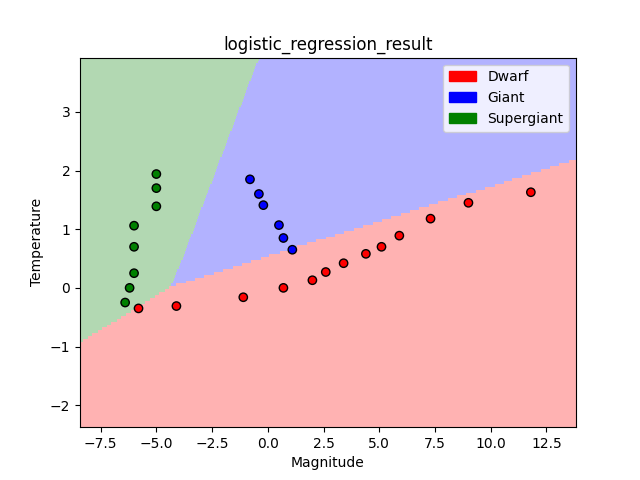
\includegraphics[scale = 0.75]{logistic_regression_result.png} \\
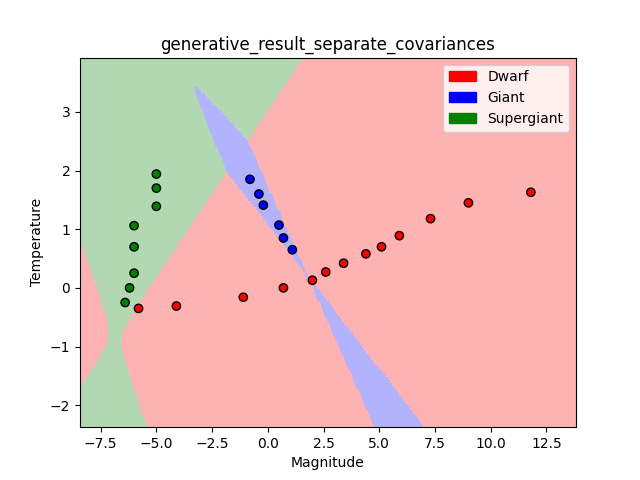
\includegraphics[scale = 0.75]{generative_result_separate_covariances.png} \\
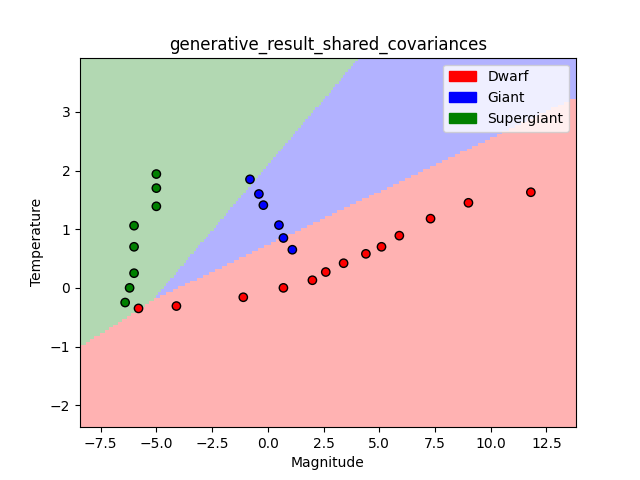
\includegraphics[scale = 0.75]{generative_result_shared_covariances.png} \\
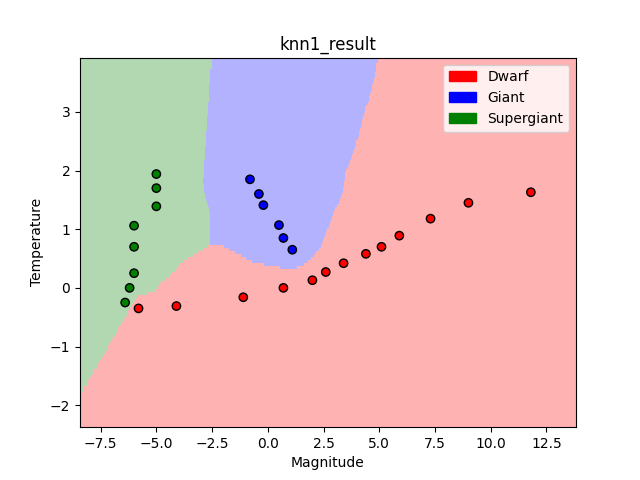
\includegraphics[scale = 0.75]{knn1_result.png} \\
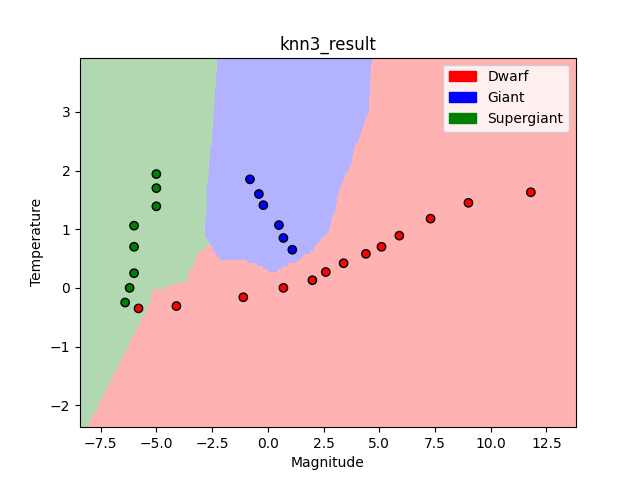
\includegraphics[scale = 0.75]{knn3_result.png} \\
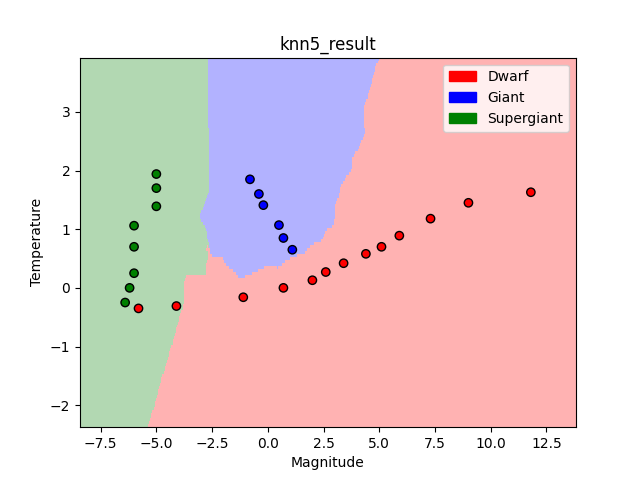
\includegraphics[scale = 0.75]{knn5_result.png} \\
\end{center}
Of the classifiers, we observe that the logistic regression and Gaussian generative models with shared covariance classify similarly and have the most simple linear decision boundaries. The Gaussian generative model with separate covariances classifies in a distinct manner from all other classifiers and has more complicated and unique decision boundaries.
The kNN classifiers have decision boundaries that loosely resemble those of the logistical regression and Gaussian generative models but have jagged-nonlinear decision boundaries.  \\ \\
The differences between these classifiers can be explained by the different implementations of each classifier. 
The logistic regression and Gaussian generative models with shared covariance are the most simplified/generalized classifiers and thus have the most simple decision boundaries. The logistic regression classifier utilizes regularization to simplify regression lines while the Gaussian generative model uses a shared covariance for for the Gaussian class-conditional densities of all data points. By comparison, the Gaussian genarative model with separate covariance has more complex decision boundaries as each class has its own covariance matrix for the Gaussian class-conditional densities. \\ \\
The jagged decision boundaries of the kNN classifiers make sense as classification relies on proximal training data points, whose positions are distributed in a sporadic nonlinear manner. As the value of $k$ increases, we see these classifiers start to misclassify at the boundary between Dwarf and Supergiant ($k=3$, $k=5$). This is due to the influence of more points in classification. Since there are more Supergiant training data points close to the boundary than there are Dwarf training data points, as $k$ increases, classification at this boundary is skewed more and more towards the Supergiant class.
\subsection*{Solution 3.2:}
\begin{center}
    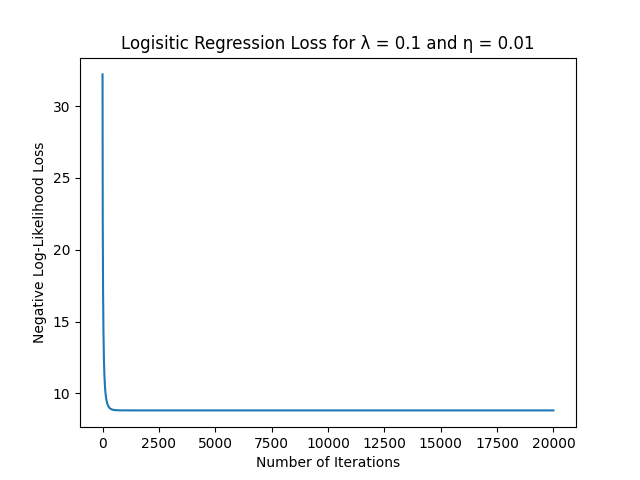
\includegraphics[scale = 0.5]{loss.png}
\end{center}
\\ \\
My choices for learning rate and regularization strength were $\eta = 0.01$ and $\lambda = 0.01$. These choices were reasonable as they helped minimize the loss of our model in the least number of iterations across all other choices.  \\ \\
Increasing the learning rate caused too large a step size, leading the gradient descent algorithm to continually overshoot the ideal update of our parameters by taking too large a step in the opposite direction of the gradient, making it near impossible to converge and resulting in high loss. On the flip side, decreasing the learning rate caused too small of a step size that we were not making significant enough updates to our parameters through each to actually improve the model, meaning the rate of convergence was very slow and also resulting in more loss. \\ \\
For the regularization strength, using too large of a strength leads our model to become unresponsive to data, incurring high bias and leading to higher loss. On the other hand, using too low of a strength leads to higher variation where the model overfits the data and does not generalize well, leading to higher loss on data outside the training set.
\subsection*{Solution 3.3:}
For negative log-likelihood of the model with separate covariance I had 64.173 while for the model with shared covariance, I had 116.572. The model with separate covariance has lower loss. This is because the model uses a different covariance matrix for each class, allowing it to fit a matrix with lower covariances to classes with data that is less spread (Giand and Supergiant) while fitting a matrix of higher covariances to classes with more spread out data points (Dwarf), leading it to incure less negative log-likelihood loss. On the other hand, the shared covariance model uses the the same covariance on all classes and thus incurs more loss. 
\subsection*{Solution 3.4:}
This star was classified as a Dwarf by all classifiers except the logistic regression model and Gaussian generative model with shared covariance, which classified it as a Giant. This is likely because these two models have the most simplified linear decision boundaries. While there is not any data from the training set to compare the correctness of either classification, the classifiers with more complex decision boundaries seem to overfit the model and more skewed towards the training data, leading me to be more skeptical of their classifications. As such, I would be inclined to trust the more genarlized logistic regression model and Gaussian generative model with shared covariance classification.
\newpage
%%%%%%%%%%%%%%%%%%%%%%%%%%%%%%%%%%%%%%%%%%%%%
% Name and Calibration
%%%%%%%%%%%%%%%%%%%%%%%%%%%%%%%%%%%%%%%%%%%%%
\subsection*{Name}

Jamin Liu

\subsection*{Collaborators and Resources}
Whom did you work with, and did you use any resources beyond cs181-textbook and your notes?

\subsection*{Calibration}
Approximately how long did this homework take you to complete (in hours)?
\\ \\
20


\end{document}
